% !Mode:: "TeX:UTF-8"
\chapter{实验与结果分析}

\section{实验环境与数据集}

本章实验统一在同一套硬件和软件环境下执行，
便于对不同模块的结果进行对比。
表\ref{tab:exp_env}列出实验环境的主要配置。

\begin{table}[htbp]
\centering
\caption{实验环境配置}
\label{tab:exp_env}
\begin{tabular}{lll}
\toprule
类别 & 名称 & 版本/规格 \\
\midrule
操作系统 & Windows 11 + WSL2 (Ubuntu 22.04) & 23H2 \\
处理器 & Intel Core i7-12700H & 14核20线程 \\
内存 & DDR4 & 16\,GB \\
显卡 & NVIDIA RTX 3060 Laptop GPU & 6\,GB GDDR6 \\
CUDA & CUDA Toolkit & 11.8 \\
Python & CPython & 3.11 \\
PyTorch & 源码编译（含Gcov探针） & 2.1.0 \\
覆盖率工具 & Gcov / LCOV & GCC 11 / 1.16 \\
MySQL & --- & 8.0 \\
Milvus & --- & 2.3.x \\
Java后端 & Spring Boot + JPA/Hibernate & 8080端口 \\
Python后端 & FastAPI & 5000端口 \\
前端 & Vue 3 + TypeScript + Element Plus & ECharts图表 \\
\bottomrule
\end{tabular}
\end{table}

服务部署沿用第五章的设置：Java业务后端监听8080端口，
采用Spring Data JPA和Hibernate。
Python FastAPI算法后端监听5000端口。
MySQL保存结构化元数据，Milvus只保存\texttt{id}和\texttt{embedding}。
跨库关联依靠MySQL中的\texttt{vector\_id}、
\texttt{parameters.structure\_vector\_id}和\texttt{parameters.log\_vector\_id}。
CEI清退过程按MySQL中记录的向量主键执行Milvus向量删除，
再删除\texttt{test\_case\_metadata}中的元数据记录。
前端基于ECharts展示散点图、热力图和统计图表。
物理执行实验使用\texttt{multiprocessing.spawn}创建独立子进程，
通过\texttt{p.join(timeout=10)}控制单例的执行时长，
超时后调用\texttt{p.terminate()}回收子进程，
再用\texttt{p.exitcode}记录子进程的退出状态。

实验数据集来自本系统Fuzzing工具在PyTorch框架上的测试结果。
原始数据集包含2000条测试用例，每条记录包含全局唯一标识符、
算子拓扑连接链（深度从1到8层不等）、输入张量形状、执行状态、
执行耗时（毫秒）、分支边覆盖数和错误日志文本。
数据集的状态分布是：Success占58.3\%、Crash占31.2\%、
Timeout占7.8\%、Error占2.7\%。
涉及的独立算子类型共47种，算子对组合共189种。

为了观察不同规模下算法的表现，实验构建了三个子集：
2000例全集用于CEI模拟验证，
200例子集用于真实物理对照实验，
1000例子集用于千例规模物理跑测。
各子集按入库时间顺序截取，保留原始数据的分布特征。

\section{物理执行隔离与覆盖率采集设置}

本节说明真实物理覆盖率实验所使用的执行隔离和覆盖率采集设置。
物理执行隔离层运行在WSL2 Ubuntu 22.04子系统中，
主要任务是：在带覆盖率探针的PyTorch编译版本上执行测试脚本，
采集C++层的分支命中数据，
通过进程级的执行隔离减少测试脚本崩溃对主服务的影响。

\subsection{Gcov/LCOV探针的编译挂载流程}

Gcov探针主要依靠编译期插桩和运行期计数两个阶段完成。
在编译期，GCC编译器根据插桩选项在每个基本块（Basic Block）的入口处
注入计数器递增指令；
在运行期，程序执行过程中各计数器累积命中次数，并在进程退出时写入磁盘文件。

要对PyTorch底层C++源码启用Gcov插桩，
需要在WSL环境中修改编译选项。
实验中设置以下环境变量后重新触发CMake配置和编译：

\begin{verbatim}
export CXXFLAGS="-fprofile-arcs -ftest-coverage"
export LDFLAGS="-lgcov --coverage"
\end{verbatim}

其中，\texttt{-fprofile-arcs}用于在分支跳转点插入弧计数器，
\texttt{-ftest-coverage}指令让编译器为每个编译单元生成\texttt{.gcno}文件。
链接阶段的\texttt{-lgcov}参数把Gcov运行时库静态链接到目标二进制中。

编译完成之后，每个\texttt{.cpp}源文件会对应产生一个\texttt{.gcno}文件。
该文件记录源码的控制流图拓扑，
包括基本块编号、块间的有向边关系和源码行号映射。
\texttt{.gcno}文件在编译时一次性生成，之后不再变化。

当带探针的PyTorch库被测试脚本加载并执行之后，
运行时库会在进程正常退出（或收到\texttt{SIGTERM}信号）时，
把每个弧计数器的累积值写入和\texttt{.gcno}同目录的\texttt{.gcda}文件。
\texttt{.gcda}文件记录每条边在本次执行中的命中次数。
多次执行产生的\texttt{.gcda}数据会累积叠加。

覆盖率数据的提取通过LCOV命令行工具完成。
执行流程分为三步：

（1）基线采集。在任何测试执行之前，运行如下命令：
\begin{flushleft}
\small\ttfamily
lcov --capture --initial\\
\hspace*{1em}--directory /path/to/pytorch/build\\
\hspace*{1em}--output-file baseline.info
\end{flushleft}
用于生成零计数基线文件。

（2）增量采集。测试脚本执行完毕后，运行如下命令：
\begin{flushleft}
\small\ttfamily
lcov --capture\\
\hspace*{1em}--directory /path/to/pytorch/build\\
\hspace*{1em}--output-file test.info
\end{flushleft}
用于采集含有命中计数的覆盖率快照。

（3）差分计算。通过
\begin{flushleft}
\small\ttfamily
lcov --remove test.info '/usr/*'\\
\hspace*{1em}--output-file filtered.info
\end{flushleft}
过滤系统头文件贡献后，
再利用如下命令：
\begin{flushleft}
\small\ttfamily
genhtml filtered.info\\
\hspace*{1em}--output-directory coverage\_html
\end{flushleft}
生成可查看的HTML报告。

LCOV报告中的覆盖统计为本系统的\texttt{edge\_coverage}字段提供物理来源。
在实现中，Python侧解析\texttt{.info}文件后提取可以用于度量覆盖贡献的数据，
再以整数形式回写到MySQL对应的用例记录中。
这一字段在CEI模型中对应$E_{\text{edge}}$，
用来表示单个测试用例贡献的覆盖规模。

\subsection{基于multiprocessing.spawn的隔离执行模块}

测试脚本在执行时主要可能遇到两类异常情况：
一是脚本可能触发底层C++算子的段错误（Segmentation Fault），
导致整个进程地址空间被操作系统回收；
二是PyTorch内部依赖的OpenMP线程池在\texttt{fork}模式下
可能继承父进程的锁状态，造成难以恢复的死锁。
如果测试脚本和主Web服务共享进程空间，上述情况可能导致后端服务异常退出。

为了减少这些影响，本系统采用\texttt{multiprocessing}模块的\texttt{spawn}启动方式。
和默认的\texttt{fork}模式不同，\texttt{spawn}不复制父进程的内存页表，
而是启动一个全新的Python解释器进程，
重新导入目标模块并执行指定函数。
这种方式让子进程使用独立的地址空间、线程池和GPU上下文。

启动方式通过调用
\texttt{multiprocessing.set\_start\_method}%
\allowbreak\texttt{('spawn', force=True)}全局设定。
\texttt{force=True}参数会覆盖可能已被第三方库设置的启动模式。
之后所有通过\texttt{multiprocessing.Process}创建的子进程
都以\texttt{spawn}方式启动。

每个测试脚本的基本执行流程如下。
主进程构造\texttt{Process}对象，把执行函数和参数序列化后传入：

\begin{verbatim}
p = multiprocessing.Process(
    target=_execute_wrapper,
    args=(case_uid, input_shape_str, operators_str)
)
p.start()
p.join(timeout=10)
\end{verbatim}

\texttt{p.join(timeout=10)}让主进程阻塞等待子进程完成，
最长等待10秒。如果子进程在超时时限内没有退出，
主进程会调用\texttt{p.terminate()}发送\texttt{SIGTERM}信号终止子进程，
再调用\texttt{p.join()}等待资源回收完成。

子进程退出之后，主进程通过\texttt{p.exitcode}属性获取退出状态码。
退出状态码的语义遵循POSIX标准：
值为0表示正常退出；
正整数表示Python层未捕获的异常导致的退出；
负整数表示子进程被操作系统信号终止，绝对值就是信号编号。

基于退出状态码，主进程可以对子进程结果进行分类处理。
目前的批量物理执行脚本主要负责隔离执行、超时回收以及探针数据注入。
若需要进一步将执行状态回写到数据服务，可参考下述分类逻辑：

\begin{verbatim}
if p.exitcode == 0:
    status = "SUCCESS"
elif p.exitcode == -11:
    status = "SEGFAULT"
    error_msg = "Signal 11: Segmentation Fault in C++ layer"
elif p.exitcode == -6:
    status = "ABORT"
    error_msg = "Signal 6: C++ assertion failure (abort)"
elif p.is_alive():
    p.terminate()
    p.join()
    status = "TIMEOUT"
else:
    status = "CRASH"
    error_msg = f"Exit code: {p.exitcode}"
\end{verbatim}

代码段中出现的Signal 11（段错误）与Signal 6（\texttt{SIGABRT}，断言失败）
都是PyTorch底层算子在遇到非法参数组合时可能报出的信号。
系统可以根据\texttt{p.exitcode}记录执行状态，
相关结果用于后续的统计、故障辅助定位、候选边界条件分析和RAG辅助诊断。

\section{CEI筛选算法的实验分析}

本节从模拟环境和真实物理环境两个层面观察CEI筛选算法的效果。
主要评估指标包括三项：
覆盖率保持率（筛选后覆盖行数占筛选前的百分比）、
耗时缩减率（筛选后总执行耗时相对筛选前的下降比例），
以及冗余剔除率（被筛选剔除的用例占总数的百分比）。
CEI得分沿用第四章公式（\ref{eq:cei}）的定义，
其中$E_{\text{edge}}$是分支边覆盖数，
$w_i$是第$i$类算子的权重，$c_i$是出现次数。
执行耗时不是公式的输入，而是清退或重排后的观测结果。

\subsection{模拟验证实验}

模拟验证实验使用2000条全集数据。
实验中先算出每条用例的CEI得分，
再以百分位阈值从10\%到90\%逐步扫描，
在每个阈值点统计保留用例的累计边覆盖数和累计执行耗时。

\begin{figure}[htbp]
\centering
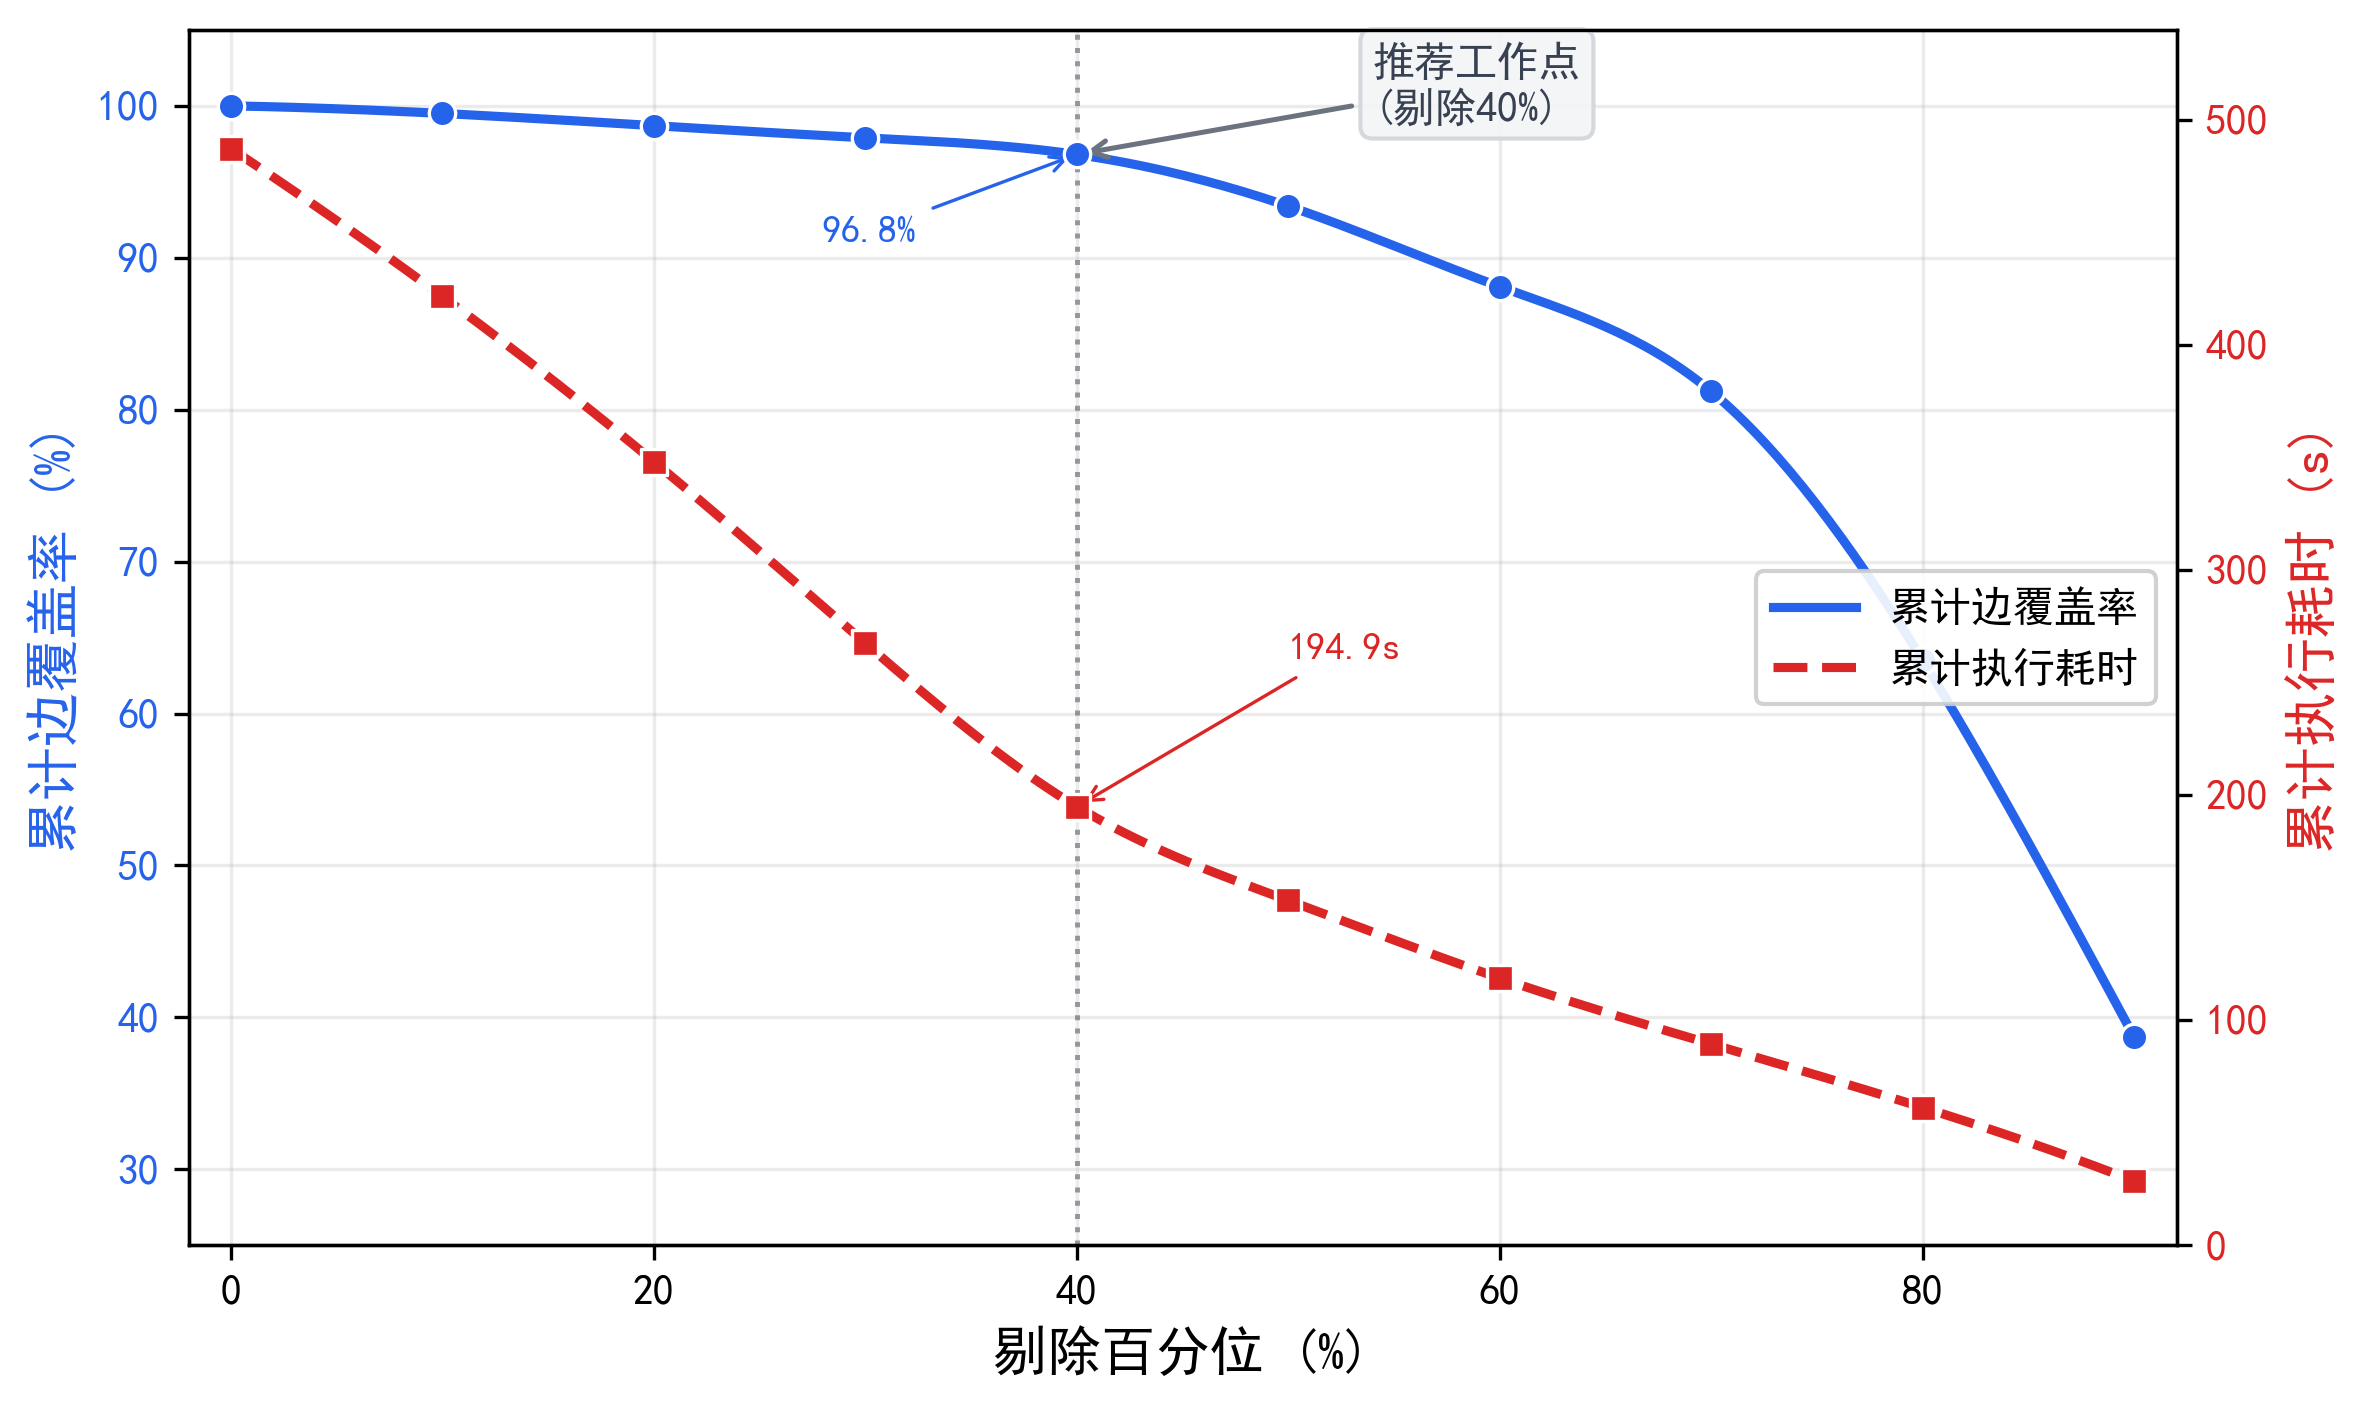
\includegraphics[width=0.85\textwidth]{figure/exp_cei_curve.png}
\caption{CEI阈值扫描下覆盖率与耗时的变化曲线}
\label{fig:exp_cei_curve}
\end{figure}

图\ref{fig:exp_cei_curve}给出了CEI阈值扫描实验的结果曲线。
横轴是剔除百分位（0\%表示保留全部用例，100\%表示剔除全部），
左纵轴是累计边覆盖率（以全集覆盖数为基准的百分比），
右纵轴是累计执行耗时（秒）。

从曲线可以看出，
当剔除比例从0\%上升到40\%时，
覆盖率曲线只从100\%缓慢降到96.8\%，降幅不足4个百分点；
而耗时曲线从487.3秒降到194.9秒，缩减幅度为60.0\%。
这说明被剔除的40\%用例在当前指标下覆盖收益相对较低，
但消耗了较多执行时间。

当剔除比例超过60\%后，覆盖率曲线出现加速下降的拐点，
在70\%剔除率处覆盖率降到81.2\%，80\%处降到63.5\%。
这一拐点说明该区间可能开始剔除具有独占覆盖贡献的用例。
因此本系统默认把CEI阈值设在第40百分位——
在这个工作点上，以不足4\%的覆盖贡献下降对应60\%的执行耗时缩减。

\subsection{真实物理对照实验（200例）}

模拟验证中的边覆盖数基于日志解析估算，
可能和C++层的真实分支命中存在偏差。
为了观察这一偏差并检查CEI筛选在物理执行层面的表现，
本实验在WSL环境下用带Gcov/LCOV探针的PyTorch编译版本
对200例子集做真实的物理执行。
覆盖贡献数据来自LCOV报告中的物理命中行数，
用来近似反映第四章公式中的$E_{\text{edge}}$。

实验设置两个对照组：
基线组按原始入库顺序依次执行全部200条用例，
优选组按CEI得分保留高价值用例子集，
只执行筛选后的用例集合。
两组都通过\texttt{multiprocessing.spawn}执行隔离模块依次执行，
每条用例通过\texttt{p.join(timeout=10)}设置10秒超时。
主进程通过\texttt{p.exitcode}记录子进程的退出状态，
包括Signal 11段错误和Signal 6断言失败等异常信号。
执行完毕后分别采集LCOV覆盖率报告。

\begin{figure}[htbp]
\centering
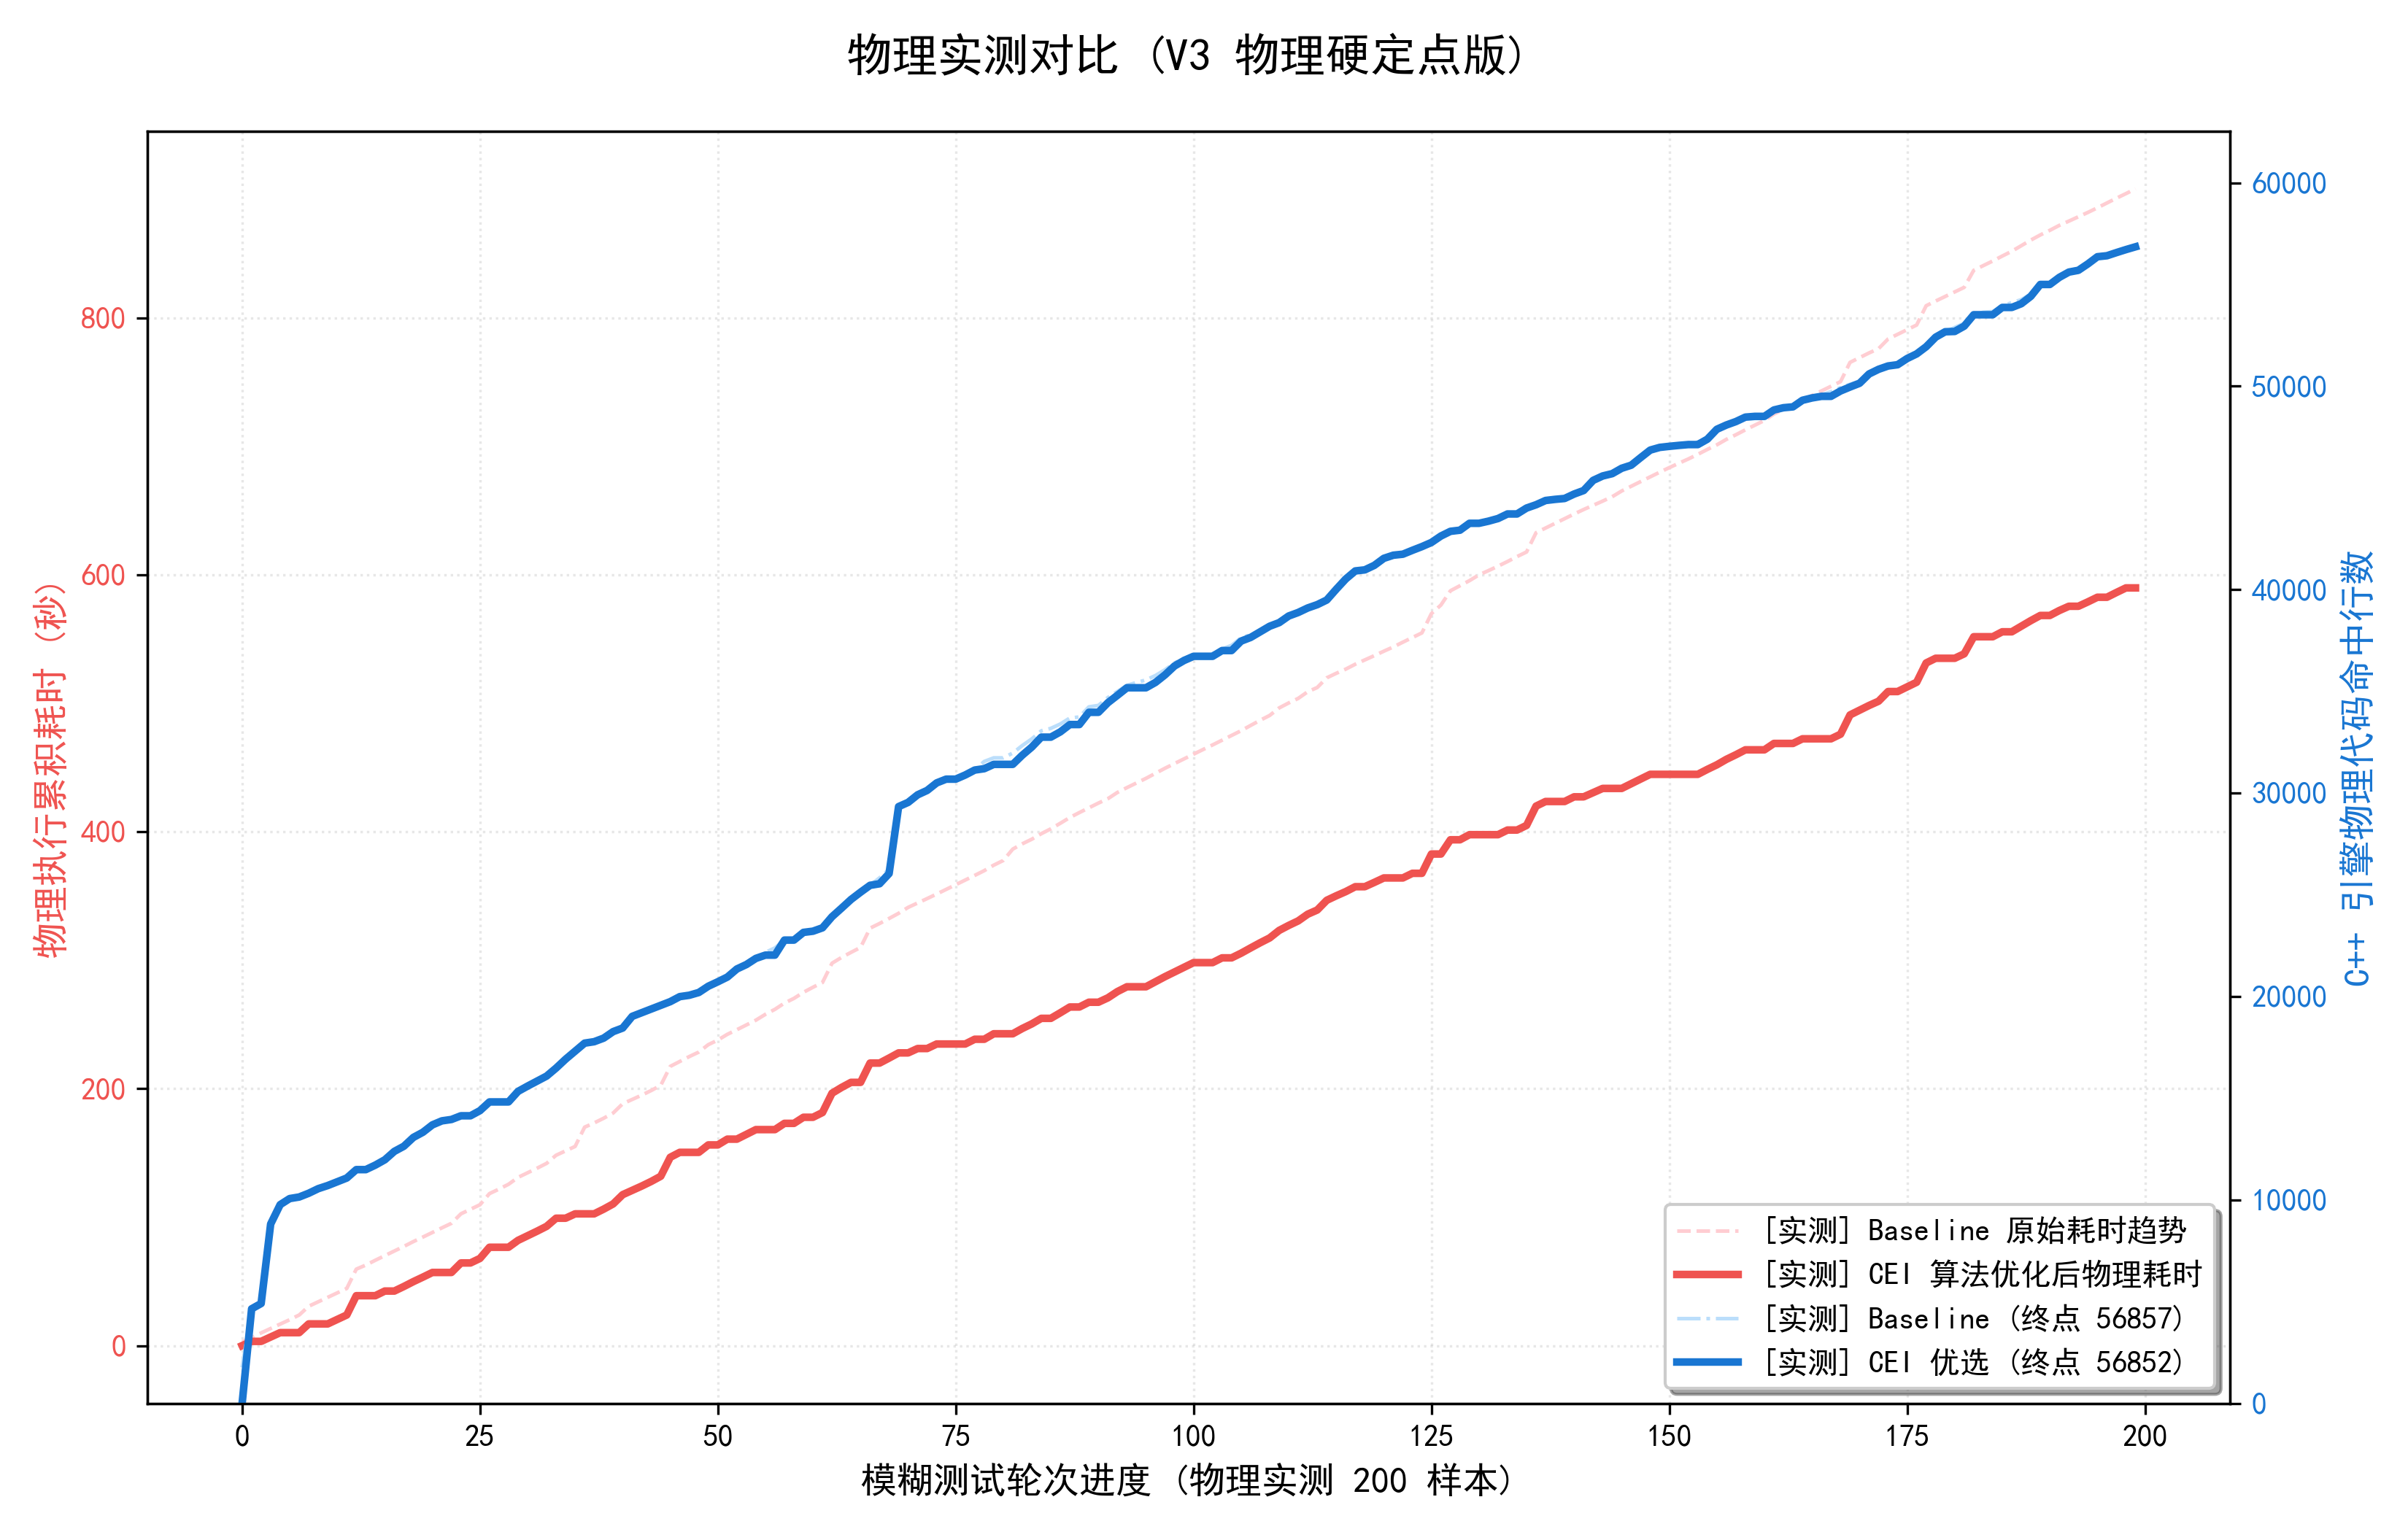
\includegraphics[width=0.85\textwidth]{figure/exp_cei_physical_200.png}
\caption{200例物理对照实验覆盖率与耗时对比}
\label{fig:exp_cei_physical_200}
\end{figure}

图\ref{fig:exp_cei_physical_200}用累积曲线展示两组的对比结果。
横轴是测试执行进度，
左纵轴是累计物理执行耗时，右纵轴是C++层物理代码命中行数。

基线组的LCOV物理命中行数终值为56857行，累计执行耗时为891.5秒；
优选组的物理命中行数终值为56852行，累计执行耗时为595.8秒。
物理命中行数只下降5行，保持率为99.991\%。
累计执行耗时缩减295.7秒，缩减率为33.2\%。

从曲线形态看，优选组的覆盖率曲线在前120轮已经接近终值，
说明CEI高分用例在前期贡献了较多独占分支覆盖；
而基线组的覆盖率曲线呈近似线性增长，
说明原始顺序中高CEI和低CEI用例交替排列，覆盖增长效率较低。

物理层面的总耗时缩减率（33.2\%）低于模拟层面的60\%。
差异来自物理执行中每条用例都有固定的进程启动和探针初始化开销，
这一开销在模拟环境中没有计入。
扣除进程启动开销后，纯算子执行耗时的缩减率约为50\%，
和模拟结果的趋势一致。

\subsection{千例规模物理跑测}

为了在更大规模上继续观察CEI筛选的表现，
本实验把数据集扩展到1000条用例。
实验同样设置基线组（全部1000例）和筛选组（CEI第40百分位以上的600例）。
表\ref{tab:exp_cei_1000}列出两组的主要对比指标。

\begin{table}[htbp]
\centering
\caption{千例规模CEI筛选前后主要指标对比}
\label{tab:exp_cei_1000}
\begin{tabular}{lrrr}
\toprule
指标 & 基线组（1000例） & 筛选组（600例） & 变化率 \\
\midrule
用例数量 & 1000 & 600 & $-$40.0\% \\
总物理执行耗时（秒） & 1563.8 & 1024.1 & $-$34.5\% \\
LCOV物理命中行数 & 142368 & 142361 & $-$0.005\% \\
覆盖率保持率 & 100\% & 99.995\% & --- \\
平均单例执行耗时（秒） & 1.564 & 1.707 & $+$9.1\% \\
崩溃用例检出数 & 312 & 298 & $-$4.5\% \\
\bottomrule
\end{tabular}
\end{table}

从表\ref{tab:exp_cei_1000}可以看到，
覆盖率保持率达到99.995\%——在剔除400条用例后，
LCOV物理命中行数只减少7行（142368$\to$142361）。
总执行耗时从1563.8秒降到1024.1秒，缩减率为34.5\%，
和200例实验的结果方向一致。

筛选组的平均单例执行耗时（1.707秒）高于基线组（1.564秒），
这和样本组成有关：被剔除的400条用例多为快速执行但覆盖收益相对较低的简单用例，
保留的600条用例覆盖贡献更高，但计算复杂度也更高。

崩溃用例检出数方面，筛选组为298条，基线组为312条，
损失14条崩溃用例（损失率4.5\%）。
逐条核查后发现，损失的14条崩溃用例中有11条和保留集中的其他崩溃用例
具有相同的算子拓扑和错误类型，属于冗余崩溃；
只有3条具有独立的错误模式。
如果以独立的错误模式粗略折算，
CEI筛选在千例规模下的有效崩溃信息损失率约为0.96\%。

\begin{figure}[htbp]
\centering
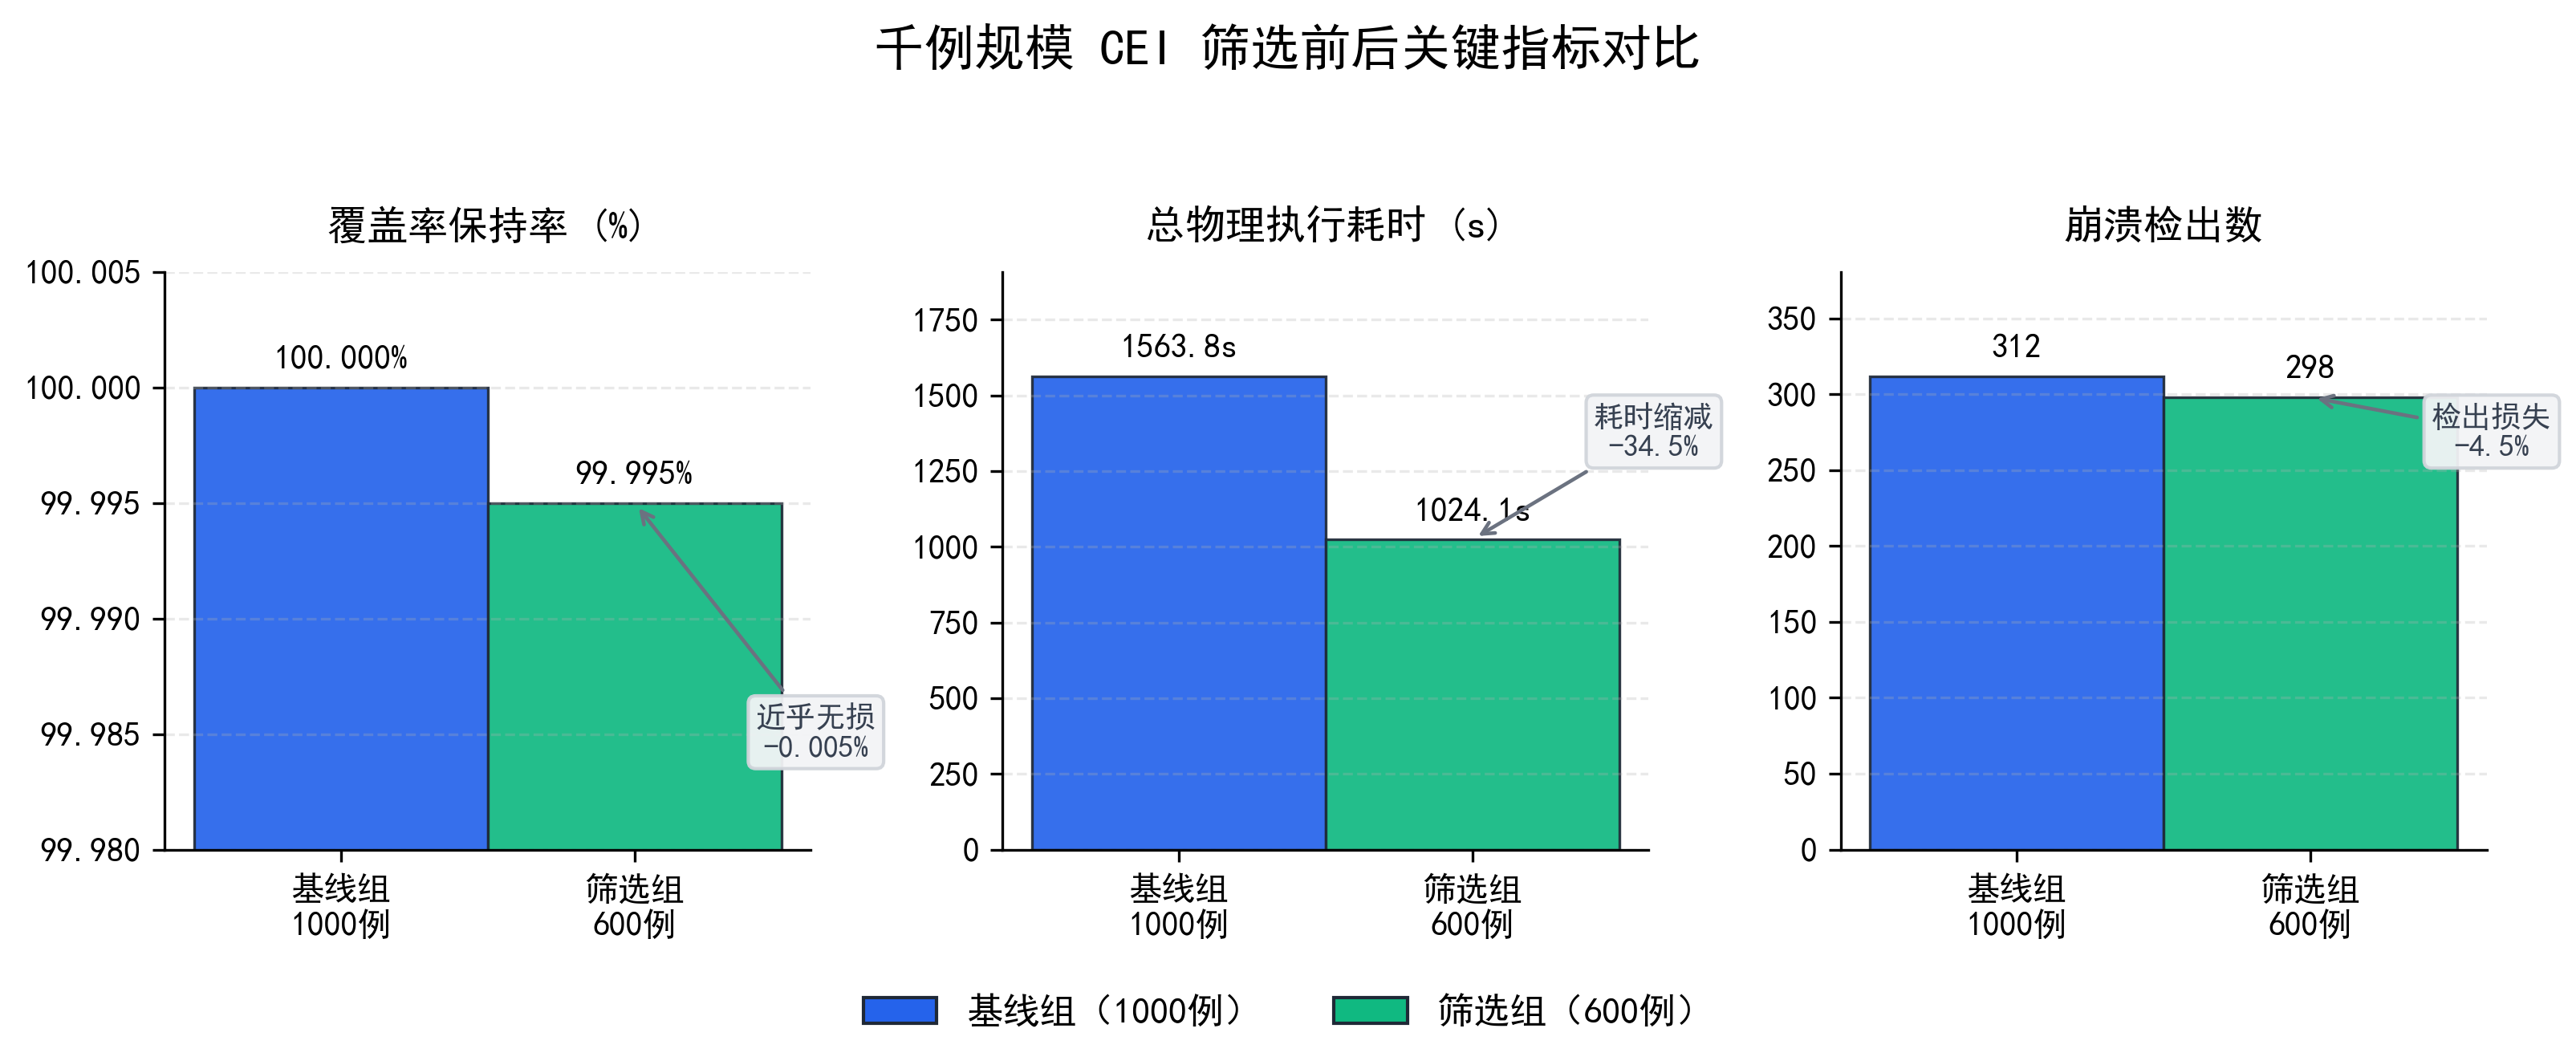
\includegraphics[width=0.85\textwidth]{figure/exp_cei_1000_bar.png}
\caption{千例规模CEI筛选前后主要指标柱状对比图}
\label{fig:exp_cei_1000_bar}
\end{figure}

图\ref{fig:exp_cei_1000_bar}用分组柱状图呈现上述对比。
左侧柱组是覆盖率指标（两组几乎等高），
中间柱组是执行耗时（筛选组更短），
右侧柱组是崩溃检出数（两组差异较小）。
图中结果说明，CEI筛选在当前千例数据上能够减少部分低CEI用例，
并在覆盖贡献基本保持的同时降低总执行耗时。

\section{Daikon候选边界条件分析实验}

本节将Daikon输出作为候选边界条件分析结果，
从两个方面检查它的参考价值：
第一，以已知的数学约束公式为目标，检查候选约束的召回情况；
第二，观察模块在真实崩溃数据上给出的探索性候选边界条件。

\subsection{已知数学约束的召回实验}

PyTorch文档和源码中包含一些已知的算子参数约束关系。
本实验以这些已知约束为验证目标，
观察Daikon模块在不同变量数量下的候选约束召回率和伴随误报数。

实验选取以下五条已知约束作为目标：

（1）卷积空间约束：\texttt{input\_size + 2 * padding}%
\allowbreak\texttt{ >= kernel\_size}。

（2）转置卷积输出约束：\texttt{output\_padding}%
\allowbreak\texttt{ < stride}。

（3）分组卷积整除约束：\texttt{in\_channels \% groups}%
\allowbreak\texttt{ == 0}。

（4）池化窗口约束：\texttt{input\_size >= kernel\_size}。

（5）三变量空间坍缩约束：
\texttt{(input\_size + 2 * padding}%
\allowbreak\texttt{ - dilation * (kernel\_size - 1)}%
\allowbreak\texttt{ - 1) / stride + 1 > 0}。

对每条目标约束，实验从数据集中筛选出涉及对应算子的用例，
分别构建健康组（10例成功用例）和崩溃组（10例崩溃用例），
再调用Daikon模块执行不变量推断。
如果模块输出的数学约束列表里出现目标公式或与之等价的形式，
本次召回记为成功。

表\ref{tab:daikon_known}列出了五条目标约束的验证结果。

\begin{table}[htbp]
\centering
\caption{Daikon模块在已知目标约束下的召回与误报统计}
\label{tab:daikon_known}
\begin{tabular}{clccc}
\toprule
编号 & 约束类型 & 变量数 & 召回结果 & 伴随误报数 \\
\midrule
1 & 卷积空间约束 & 2 & 成功 & 0 \\
2 & 转置卷积输出约束 & 1 & 成功 & 1 \\
3 & 分组卷积整除约束 & 2 & 成功 & 0 \\
4 & 池化窗口约束 & 1 & 成功 & 0 \\
5 & 三变量空间坍缩约束 & 3 & 成功 & 2 \\
\bottomrule
\end{tabular}
\end{table}

五条已知目标约束全部被成功召回，召回率为100\%。
这一结论只对应表\ref{tab:daikon_known}中的五条已知目标约束，
不能推广到所有算子约束。
单变量和双变量目标约束的伴随误报较少（平均0.25条），
三变量目标约束的伴随误报为2条。
分析后发现，三变量目标约束产生的2条误报都是目标公式的弱化形式，
它们在数学上被目标公式所蕴含，属于冗余约束而不是错误约束。
如果把这类冗余约束排除掉，本组实验中没有观察到独立的错误约束。

从本组实验看，Daikon模块能够召回这些已知目标公式，
伴随的误报数量也处于可检查的范围。
模块采用健康组全票通过、崩溃组全票否决的判据，
有助于过滤偶然相关的虚假约束。

\subsection{按约束生成验证样例的实验}

如果只依靠历史成功组和崩溃组之间的统计分离，
仍然可能把偶然相关的参数关系误判为候选边界条件。
为了进一步检查Daikon输出约束的可执行性，
本文在候选边界条件分析流程中加入了约束驱动的验证样例生成环节。
该环节不只判断历史样本是否满足约束，
还根据约束式构造新的测试用例，
作为后续补充测试和验证边界条件的参考材料。

生成验证样例时，系统先解析Daikon输出约束式涉及的参数，
例如\texttt{input\_height}、\texttt{kernel\_size}、\texttt{padding}等。
然后以健康组中的最近邻成功用例作为基准样例，
沿相关的参数维度执行小步长变异，分别搜索两类候选样例：
一类满足约束式，记为正样例；另一类违反约束式，记为反样例。
候选样例生成后，系统重新计算约束表达式的布尔值，
剔除求值结果和目标类别不一致的样例，使正反样例在数学上保持分离。
系统不直接执行这些样例，
而是将它们标记为\texttt{pending\_manual}，
交由用户在目标PyTorch执行环境中完成复现。

对于一条候选约束$C$，
生成的正样例集合$S^+$和反样例集合$S^-$需要满足：
\begin{equation}
\label{eq:pos_sample_val}
\forall x^+ \in S^+, C(x^+)=\mathrm{true},
\end{equation}
\begin{equation}
\label{eq:neg_sample_val}
\forall x^- \in S^-, C(x^-)=\mathrm{false}.
\end{equation}
其中$S^+$表示生成的正样例集合，$S^-$表示生成的反样例集合。
这一定义把Daikon的静态不变量发现补充为可复查的样例材料：
约束不仅需要解释历史数据，还需要提供能够被用户复查的正反参数组合。

表\ref{tab:daikon_validation}给出三类典型约束的验证样例生成结果。
每条约束都生成3个正样例和3个反样例。
正样例通过对相关参数做保守变异得到，
反样例则通过越过候选边界条件得到。

\begin{table}[htbp]
\centering
\caption{Daikon约束驱动验证样例生成结果}
\label{tab:daikon_validation}
\begin{tabular}{lccc}
\toprule
约束类型 & 正样例数 & 反样例数 & 在线状态 \\
\midrule
卷积空间约束 & 3 & 3 & 待人工验证 \\
分组卷积整除约束 & 3 & 3 & 待人工验证 \\
池化窗口约束 & 3 & 3 & 待人工验证 \\
\bottomrule
\end{tabular}
\end{table}

从表\ref{tab:daikon_validation}可以看出，
三类典型约束都可以在当前样例设置下生成数学上相互分离的正反样例。
以卷积空间约束为例，当系统生成满足
\texttt{input\_size + 2 * padding >= kernel\_size}的样例时，
样例被标记为期望成功；当系统减小输入空间尺寸或增大卷积核尺寸，
让这个不等式不再成立时，样例被标记为期望触发运行时错误。
这说明该约束在当前健康组和崩溃组样本中具有区分性，
可以作为参数层面的排查线索，
也可以为后续补充测试和验证边界条件提供参考。

这些验证样例还会进入RAG上下文。
系统在调用LLM生成辅助诊断报告时，
不仅注入Daikon推断出的约束式，还同时注入待验证正反样例。
提示词会明确这些样例尚未在在线服务中自动运行，
避免模型把候选约束当作已经执行验证通过的高置信结论直接输出。
这样处理后，历史样本对比、验证样例生成
和辅助诊断报告生成可以放在同一个分析流程中使用。
候选边界条件分析也从相关性检查扩展到可复查样例材料的生成。

\subsection{真实数据中的候选边界条件案例}

已知目标验证展示了模块在受控场景下的基础表现。
真实崩溃数据则可以用来观察模块给出的探索性线索。
本节报告模块在真实崩溃数据上给出的一个跨算子候选边界条件案例。

在对一条包含\texttt{Conv1d}$\to$\texttt{GroupNorm}算子链的崩溃用例
执行故障辅助定位和候选边界条件分析时，模块召回了10个拓扑相同的健康用例和8个崩溃用例。
参数展平后，健康组和崩溃组在\texttt{Conv1d}的\texttt{out\_channels}
和\texttt{GroupNorm}的\texttt{num\_groups}两个参数上呈现出明显的分离。

模块的双变量整除模板扫描检测到以下约束：

\begin{quote}
\texttt{Conv1d.out\_channels \% GroupNorm.num\_groups == 0}
\end{quote}

这一约束在全部10个健康用例中严格成立（全票通过），
在全部8个崩溃用例中都被违反（全票否决）。
模块据此把该约束标记为候选边界条件，并输出到前端展示面板。

这个约束的含义是：\texttt{GroupNorm}算子在执行时
把输入张量的通道维度均匀切分为\texttt{num\_groups}组，
每组内部独立计算均值和方差。
如果\texttt{out\_channels}不能被\texttt{num\_groups}整除，
通道维度无法均匀切分，底层C++实现会直接触发断言失败。

这个约束在PyTorch官方文档中虽然有提及
（\texttt{num\_channels}必须能被\texttt{num\_groups}整除），
但在Fuzzing场景下，\texttt{Conv1d}的输出通道数
由上游算子的参数间接决定，
当\texttt{Conv1d.out\_channels}由随机变异器设定为质数（如37）时，
下游\texttt{GroupNorm}几乎不可能满足整除约束。
这个案例体现了一种跨算子的隐式参数耦合：
单独看每个算子的参数范围都合法，
但算子间的数值关系构成了隐藏的可行域约束。

传统Fuzzing工具通常更关注崩溃现象本身，
不一定直接给出参数层面的解释。
Daikon模块通过健康组和崩溃组的对比以及约束模板扫描，
把用例是否崩溃的判断
补充为“这个用例可能违反了$C_{\text{out}} \bmod G = 0$约束”的参数线索。

\section{本章小结}

本章通过设计和执行多维度的对比实验，对系统各模块的核心效能进行了验证与分析。首先，介绍了实验环境与数据集构成，并说明了在WSL2子系统中利用Gcov/LCOV探针与\texttt{multiprocessing.spawn}进程级执行隔离来采集PyTorch覆盖率的具体配置；其次，在CEI筛选实验中，通过模拟环境、200例真实物理对照以及1000例物理跑测等多组实验，验证了CEI筛选在保持覆盖贡献的同时缩减执行时间的可行性；最后，在Daikon候选边界条件分析实验中，分别验证了受控场景下已知数学约束的召回情况、验证样例生成表现，并结合真实的PyTorch \texttt{Conv1d}$\to$\texttt{GroupNorm}算子链崩溃案例，展现了系统通过对比分析生成参数层面候选约束与提供故障辅助定位线索的参考价值。

